%!TEX root = ../dissertation.tex
\begin{savequote}[75mm]
Even two shoes in the box are correlated!
\qauthor{Dr. Alexander Lukin}
\end{savequote}

\chapter{Correlations, Entanglement, \newline and Quantum Phase Transitions} 
\label{sec:ch3}

Phase transitions, classical or quantum, are a celebrated paradigm in physics for describing the macroscopic properties of many-body systems independent of their microscopic parameters. These phases are described by a canonical diagram that distinguishes between an ``ordered" and ``disordered" macroscopic phase of the system via a quasi-local observable known as an ``order parameter". This parameter possesses a non-zero value in the ``ordered" regime and becomes zero when it enters the ``disordered" regime. The transition of the macroscopic system from one phase to another is often performed by tuning a thermodynamic constraint such as the equilibrium temperature of the system: the solid to liquid transition at the melting point, the ferromagnetic to paramagnetic transition at the Curie point, or the condensing of bosonic atoms into a Bose-Einstein condensate (BEC) at the critical temperature of a trapped, ultracold atomic gas \cite{Pethick2002,Sachdev2011,Kardar2012a,Kardar2012b}. 

%This transition occurs at a critical point of this tuning parameter between the two phases and describes where the order parameter becomes non-zero.

In classical systems, these thermodynamic transitions occur at a particular temperature when the thermal energy per constituent is comparable to a microscopic interaction parameter that governs the ordering of the system. This leads to a non-analyticity of the thermodynamic free energy and defines the point of the phase transition \cite{Kardar2012a,Kardar2012b}. The ability of the system to actually change its macroscopic ordering requires that the system possesses microscopic fluctuations, in this case driven by the microscopic thermal fluctuations that accompany a given temperature. The ability of these fluctuations to drive the system from a disordered state towards an ordered one requires the correlation of these fluctuations across the system such that they bring the system collectively towards a macroscopically ordered state. As such, a length scale can be defined that associates the spatial extent of these correlations in the system and gives rise to many of the characteristic associations with phase transitions such as the correlation length diverging at the critical point. This divergence of correlations at the critical point represent, perhaps, one of the best examples of a many-body system that cannot be accurately described by only looking at a few of its microscopic constituents.

The most remarkable aspect of this phase transition paradigm being that, while many phase transitions may differ in absolute values, their qualitative scaling behaviors for such transitions depend only upon a few global constraints such as dimensionality or underlying symmetries. This means that given some appropriate rescaling of different systems, their macroscopic (thermodynamic) behavior will be identical and therefore the behavior of the transition is actually ``universal". 

\begin{figure}[t!]
		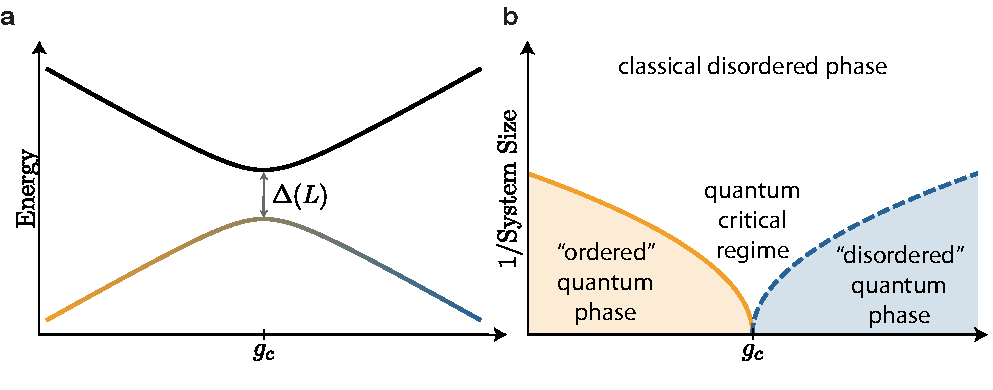
\includegraphics[width=\columnwidth]{figures/ch3/qptv2edit.pdf} 
		\caption{\textbf{Schematic of a Quantum Phase Transition. a)}  The canonical schematic for a quantum phase transition occurring at $T=0$ for the ground state as a function of a tuning parameter $g$. The avoided crossing shown between the ground state and the excited state in this diagram are separated by the coupling between the two terms in the Hamiltonian:  $H_0$ and $H_1$. Each dominating character of the ground state in their respective regimes. The color of the ground state denotes whether it lies in the ``ordered" or ``disordered" phase. \textbf{b)}  The canonical phase diagram associated for a quantum phase transition has an ``ordered" and a ``disordered" phase that cross at a critical point $g_c$ when $T=0$ and the size of the system is very large (referred to the ``thermodynamic limit"). The left diagram, \textbf{a}, is a plot of the eigenstates along a finite system size cross section of this diagram. As the system size is increased, this gap goes to zero. As the temperature is increased, more eigenstates in the system become incoherently populated and conceptually the quantum fluctuations, $\hbar \omega_c$, that attempt to order the system compete with the thermal fluctuations $k_\text{B} T$ that drive the system towards a disordered phase.  The closing gap near the critical point extends this classically disordered phase downward into the critical ``fan" shape associated with critical behavior and quantum phase transitions.}
		\label{fig:qpt}	
\end{figure}

Many of these concepts from classical phase transitions can be related to quantum phase transitions. The study of quantum phase transitions involves the tuning of a coupling parameter, $g$, in a Hamiltonian between two non-commuting terms as schematically shown in: 

\begin{equation}
\label{eqn:gHam}
H= H_0 + g H_1
\end{equation}

where $ [H_0,H_1]\neq0$. The transition of this system occurs at a critical coupling point $g_c$ and is only considered at equilibrium which can occur even when $T=0$. \footnote{It is at this point, the assumption of a system at equilibrium and $T=0$, that all quantum phase transitions are typically assumed to refer to the transition in the ground state properties.} Fundamentally, the system still needs fluctuations even at $T=0$ to allow for the macroscopic ordering at the phase transition. The difference being that these fluctuations are now driven as purely ``quantum" fluctuations that persist even at $T=0$ due to the Heisenberg uncertainty principle. These quantum fluctuations also lead to a divergence in a correlation length across the system at the critical point. The question that then naturally arises is ``how much are these correlations purely quantum?" This notion of uniquely quantum correlations is intimately related to the concept of entanglement in quantum systems -- perhaps the most celebrated hallmark of ``quantum-ness." In some cases, the entropy induced in a system due to its entanglement has been used to distinguish the uniquely quantum aspect of these phase transitions. Analytical and numerical results for this entanglement behavior have been studied theoretically for both spin systems (Ising and Heisenberg models) and lattice models of itinerant particles (bosonic and fermionic) \cite{Amico2008, Osterloh2002,Osborne2002}.

This mapping of the language and Landau-Ginzburg framework of phase transitions, however, does not apply ubiquitously to all quantum phase transitions. Notably, in the case of fractional quantum hall states\cite{Kitaev2005,Levin2006,Jiang2012} or spin liquids\cite{Zhang2011,Isakov2011} their is not a clear notion of a local order parameters that distinguishes these phases, but rather their non-local entanglement that captures their behavior. 

This section will start off with a generic discussion about correlations and entanglement in quantum systems. The presence of such correlations and their relation to quantum phase transitions will be discussed in the context of experiments measuring  entanglement in the superfluid-to-Mott-insulating transition in the Bose-Hubbard model and the paramagnetic-to-ferromagnetic transition in the transverse Ising model -- both of which are realized in one dimension. While the transverse Ising model will harbor much of the generic behavior discussed above, the Bose-Hubbard model in one dimension belongs to the class of topological BKT-type transitions.

\section{Coherent superposition and statistical distributions} \label{sec:superPos}

This section provides the mathematical formalism and concepts that naturally arise in the context of correlations and entangled states. For simplicity, we start with a single-particle state to develop some intuition. If we imagine a single-spin that is prepared in the $+x$ direction, we can write it as an eigenstate of the $x$-basis or a superposition in the $z$-basis:

\[
| \rightarrow \rangle \equiv \frac{1}{\sqrt{2}} \left ( | \uparrow \rangle + | \downarrow \rangle \right )
\]

This equal superposition in the $z$-basis would result in a $50\%/50\%$ $z$-measurement distribution that would give rise to an expected average value $\langle \sigma^z \rangle = 0$. However, representing this state in this ket-vector notation actually makes an implicit assumption that the state is pure and therefore describable by a single vector that represents this coherent superposition of states in some basis. A more convenient and versatile notation that avoids this assumption is with density matrices. The density matrix for the pure state above is simply the ket-bra product:

\[
\rho = | \rightarrow \rangle \langle \rightarrow | =  \frac{1}{2} \Big ( | \uparrow \rangle \langle \uparrow | + | \uparrow \rangle \langle \downarrow | + | \downarrow \rangle \langle \uparrow | + | \downarrow \rangle \langle \downarrow | \Big )
\]

When written in matrix form where the basis states $\left \{ | \uparrow \rangle, | \downarrow \rangle \right \}$ define the row and column indices of the matrix:

\[
\rho = \frac{1}{2} \begin{bmatrix}
  | \uparrow \rangle \langle \uparrow |  & | \uparrow \rangle \langle \downarrow | \\
 | \downarrow \rangle \langle \uparrow |  & | \downarrow \rangle \langle \downarrow | \\
\end{bmatrix}\
=
 \begin{bmatrix}
 1/2 & 1/2 \\
 1/2 & 1/2 \\
\end{bmatrix}\]

The diagonal of this matrix is simply the probability of a given state outcome, in this case either$+z$ or $-z$ each happen with $50\%$ probability and give an average measured value of $ \langle \sigma^z \rangle =0$. This also implies that the diagonal must necessarily sum to unity $\mathrm{Tr} [\rho]=1$. In general then, the expectation outcome of a given observable $\hat{\mathcal{O}}$ is evaluated by the trace of the density matrix with this operator: \footnote{Conceptually, once this density matrix is written down in the measurement basis, only the diagonals of this matrix are accessible to the observer since all measurements involve a contraction with a given bra/ket-vector.}


\[
\langle \hat{\mathcal{O}} \rangle = \mathrm{Tr} [\hat{\mathcal{O}} \rho]
\]

Notably, this notation shows that a measurement along any particular, single basis (in this case the $z$-basis) is agnostic to the presence of a coherent superposition of given outcomes. In other words, the presence of the off-diagonal matrix elements does not play a role in this measurement. If, instead of $\rho = | \rightarrow \rangle \langle \rightarrow |$, we simply had a  $50\%/50\%$ statistical distribution of either $+z$ or $-z$, then our density matrix, now $\rho'$, is given by $\rho'= \frac{1}{2} | \uparrow \rangle \langle \uparrow | + \frac{1}{2} | \downarrow \rangle \langle \downarrow |$. In matrix form simply being:

\[
\rho'_z =
 \begin{bmatrix}
 1/2 & 0\\
 0 & 1/2 \\
\end{bmatrix}\]

Note that this density matrix would have all the same statistics and expectation values along the $z$-axis. However, if we were to measure along another axis, say in the $x$-basis, then we have to first rotate our state about the $y$-axis by an angle of $-\pi/2$ or simply express $|\pm z\rangle$ in the $x$-basis:

\[
 | \uparrow \rangle = \frac{1}{\sqrt{2}} \Big ( | \rightarrow \rangle + | \leftarrow \rangle \Big )
 \]
 \[
 | \downarrow \rangle = \frac{1}{\sqrt{2}} \Big ( | \rightarrow \rangle - | \leftarrow \rangle \Big )
 \]
 
 For $\rho$, we know that it is actually defined as $| \rightarrow \rangle \langle \rightarrow |$ and therefore an exact eigenstate of this measurement basis would be measured as $100\%$ in the $+x$-direction. In the case of $\rho'$, this expands to be $\rho'_x = \frac{1}{2} | \rightarrow \rangle \langle \rightarrow | + \frac{1}{2} | \leftarrow \rangle \langle \leftarrow |$, which in matrix form, is still:

\[
\rho'_x =
 \begin{bmatrix}
 1/2 & 0\\
 0 & 1/2 \\
\end{bmatrix}\]

The lack of off-diagonal, coherence terms is what differentiates this statistical distribution from before as a physically different object. This extreme case when these coherence terms are zero defines this system as a completely mixed state since the probabilities and measurements solely arise from a classical, statistical mixture of outcomes. 

A very common metric used to differentiate and quantify these two types of systems is by measuring the associated purity of a given density matrix. This purity is defined as the trace of the second moment of the density matrix: 

\begin{equation}
\label{eqn:purity}
P \equiv \mathrm{Tr} [ \rho^2]
\end{equation}

Note that this purity relies on the matrix product of $\rho$ for the second moment. In the case of a state described by a single vector, $|\psi \rangle$, this metric can easily be shown to sum to unity, since $ \rho^2 = | \psi \rangle \langle \psi | |\psi \rangle \langle \psi | = | \psi \rangle \langle \psi | = \rho$ and $\mathrm{Tr} [ \rho ] = 1$. However, in the case of a completely mixed state, such as $\rho'$, the density matrix is diagonal and so $\mathrm{Tr} [\rho_{i,i}^2]  = P < 1$ as long as there is more than one non-zero diagonal entry. The particularly powerful property of this formalism is that it is basis-independent, meaning that regardless of what basis is chosen to express the wave function or statistical mixture, the purity will give the same numerical answer\cite{nielsen2010}.

While this was a specific, single-spin example, this provides some intuition for some very general properties for physical systems that are either quantum, classical, or a mixture of both. The important implication being that the purity of a system is actually invariant under any unitary operation that can be performed on the system. One way to understand this is to think of the mixed state as a statistical mixture of different truly pure states, and as vectors with a length given by their probability, unitary operations (e.g. a rotation about an arbitrary axis) preserve this length. 

This framework of density matrices, purity, and statistical mixture provides the mathematical tools to now understand the celebrated concepts and properties associated with many-bodied wave functions. The important implication being that the constituents of the wave function can be physically separated from one another while still belonging to the same coherent many-bodied state. These same arguments from above can be applied to both the joint and local distributions such that even correlations developed among these constituents are encoded in the field of their many-bodied wave function and give rise to their uniquely quantum correlations.

\section{Correlations and Entanglement}

Entanglement is one of the most counterintuitive and truly unique consequences of quantum mechanics. It was famously shown by John Stewart Bell that entangled quantum particles can exhibit correlations that are stronger than physically possible in classical, local theories \cite{Bell1964}. \footnote{In fact, a very common question asked of any result from a quantum simulation experiment is how ``quantum" are the results. As in, how uniquely can the observed behavior be attributed to the system being a quantum one and not just one, for example, described by a classical wave theory. The violation of Bell's inequality by a system is one of these few cases that is simply unrealizable in a purely classical world.} The canonical examples of these highly entangled quantum states that exhibit such classically violating correlations are known as Bell states and were first  verified experimentally by \emph{Aspect, et al.,}\cite{Aspect1981,Aspect1982} and rule out proposed ``hidden variable" theories.  Until recently, various ``loop-holes" were brought forward as arguments such that the system could still admit a classical explanation. However, recently experiments have additionally implemented various loop-hole free versions of the Bell test\cite{Hensen2015,Giustina2015,Shalm2015} -- more stringently identifying quantum mechanics as a successful description of nature. 

% \textcolor{red}{(ADD FOOTNOTE?)}
Correlations and the presence of entanglement in a quantum system are intimately linked. For the purpose of clarity in this thesis, I will describe entanglement as a qualitative descriptor for pure, many-body quantum states that are inseparable. This inseparability means that the joint description of the quantum state is necessary and that attempting to describe the system as the product of its separated parts is insufficient. To gain some intuition about these statements, we will first consider a canonical example -- the anti-symmetric Bell state: 

\begin{equation}
\begin{aligned}
|\Psi^-\rangle = &\frac{1}{\sqrt{2}} \left (  | \uparrow_A \rangle \otimes | \downarrow_B \rangle - | \downarrow_A \rangle \otimes | \uparrow_B \rangle \right ) \\
 = & \frac{1}{\sqrt{2}} \left (  | \uparrow_A \downarrow_B\rangle - | \downarrow_A \uparrow_B \rangle \right )
\end{aligned}
\label{eqn:bellState}
\end{equation}

which is intentionally constructed to be inseparable. That is to say, that this state cannot be decomposed into a product of single-particle states of spin A and spin B, $|\Psi^-\rangle \neq |\psi_A\rangle \otimes |\psi_B\rangle$. This can additionally be seen by noting the state $| \Psi^- \rangle$ is not an eigenstate of any single-particle operator which acts only locally on the spatially separated spins. We now analyze this state to find the emergent implications of this inseparability in a quantum state composed of this two-spin state where spin A and spin B can be spatially separated. As in the previous section (\S \ref{sec:superPos}), it will again prove useful to rewrite this state as a density matrix:
%This representation of the quantum state already assumes that the system is pure and can be represented by a single vector that is in a coherent superposition of both spins pointing up or both spins pointing down.  A more convenient notation that will address the quantum versus classical states in a system is realized in the density matrix notation, which for the Bell state above is:
\begin{equation}
\begin{aligned}
\rho =  & | \Psi^- \rangle \langle \Psi^- | \\
 = & \frac{1}{2}  \Big ( | \uparrow_A \downarrow_B\rangle \langle \uparrow_A \downarrow_B | + | \downarrow_A \uparrow_B\rangle \langle \downarrow_A \uparrow_B |  - | \downarrow_A \uparrow_B\rangle \langle \uparrow_A \downarrow_B |  -
| \uparrow_A \downarrow_B\rangle \langle \downarrow_A \uparrow_B |
 \Big ) 
 \end{aligned}
 \label{eqn:bellRho}
\end{equation}

which in matrix form is expressed as:

\[
\rho = \frac{1}{2} \begin{bmatrix}
| \uparrow_A \downarrow_B \rangle \langle \uparrow_A \downarrow_B | & -| \downarrow_A \uparrow_B \rangle \langle \uparrow_A \downarrow_B |  \\
-| \uparrow_A \downarrow_B \rangle \langle \downarrow_A \uparrow_B|  & | \downarrow_A \uparrow_B \rangle \langle \downarrow_A \uparrow_B | \\
\end{bmatrix}
\]

The coefficients associated with the diagonal entries of this matrix are the joint probability outcomes of both spins for this given Bell state.  Note that $\rho$ is only showing a fraction of the total Hilbert space -- the spin configurations of $|\uparrow_A \uparrow_B\rangle, |\downarrow_A \downarrow_B \rangle$ are not written since they have zero population. 
%Expectation values of observables are then defined as the trace of this matrix multiplied by the outcomes of the observable operator, $\hat{\mathcal{O}}$, acting on a given diagonal entry $| \psi_i \rangle \langle \psi_i | $: 

As stated above, any single-particle operator (e.g. $\sigma_{A,B}^z$) changes the wave function and therefore demonstrates the state is not an eigenstate of local operators. However, there is a clear relation of the two spins in the state $| \Psi^- \rangle$ that are captured by the spin-spin correlation operator  $\hat{\mathcal{O}} = -\hat{\sigma}^z_A \hat{\sigma}^z_B$. This two-spin operator is often referred to as the total two-point correlator. \footnote{This naming convention can be a bit confusing but is common. The statistical definition for a correlator is generically written as $\frac{\langle x y \rangle - \langle x\rangle \langle y \rangle }{\sqrt{\langle x^2 \rangle - \langle x \rangle^2} \sqrt{\langle y^2 \rangle - \langle y \rangle^2}}$. This statistical definition inherently removes both offsets in the single-point measurements, $\langle x \rangle, \langle y \rangle$ and normalizes by dividing by the single-point variances. In practice for the given Bell state above, this is not necessary since the state has unit fluctuations and is centered about zero. However, later on in this thesis these distinction will become important for distinguishing between ``total", ``connected", and ``disconnected" correlations.} For the aforementioned $\rho$ we obtain $\langle \hat{\sigma}^z_A \hat{\sigma}^z_B \rangle = 1$. We can see that this correlation is significant since a single-point operator would have a value of zero, $\langle \sigma^z_{A,B} \rangle = 0$. However, measuring these correlations does not distinguish our entangled Bell state from classically correlated variables (e.g. two correlated coins that are constructed classically by a hidden operator to always flip together where one is heads and the other tails) since the measurement only relies on the diagonals. The distinguishing property of the correlations encoded in our Bell state $| \Psi^- \rangle$ is the fact it is again described by a coherent superposition; geometrically, the many-body state is again described by a single vector. 

We can explore the difference by considering a simplified test from Bell's proposal.  After preparing the two-spin state $|\Psi^-\rangle$, spin A and spin B are spatially separated and given to two different observers to be measured at the same time. Each observer is allowed to either measure their spin in the $z$ or the $x$ basis and can choose which randomly (based upon a classical random variable) as long as the observer keeps track of the result and chosen measurement axis. All of the two-spin measurements  possible are $\{ \mathcal{O}^{z,z}=- \sigma^z_A \sigma^z_B , ~\mathcal{O}^{x,z} = - \sigma^x_A \sigma^z_B, ~\mathcal{O}^{z,x}=- \sigma^z_A \sigma^x_B, ~\mathcal{O}^{x,x}=- \sigma^x_A \sigma^x_B \}$. Each joint measurement will happen with equal probability.  For the case of our Bell state $| \Psi^- \rangle$ the expectation values of these four observables after an ensemble of measurements are $\left \{ \langle \mathcal{O}^{z,z} \rangle = 1,\langle \mathcal{O}^{x,x} \rangle = 1,\langle \mathcal{O}^{x,z} \rangle = 0,\langle \mathcal{O}^{z,x} \rangle = 0 \right \}$. We could then construct some integrated quantity that combines these measurements into a single metric: e.g. $C=\frac{1}{4} \sum_{i,j\in x,z} \mathcal{O}^{i,j}= 1/2$. 

However, if we had instead shared two classically correlated spins with each observer, we would produce a mixed density matrix $\rho'$: 

\[\rho = \frac{1}{2} \begin{bmatrix}
| \uparrow_A \downarrow_B \rangle \langle \uparrow_A \downarrow_B | & 0  \\
0 & | \downarrow_A \uparrow_B \rangle \langle \downarrow_A \uparrow_B | \\
\end{bmatrix}\]

Physically, this would amount to some classical intermediary that randomly (perhaps based upon the toss of a fair coin) prepares the anti-correlated spins and gives one to either observer A or observer B. If observers A and B again perform the same random $x,z$ measurements, they would obtain the outcome $C=\frac{1}{4} \sum_{i,j\in x,z} \mathcal{O}^{i,j}= 1/4$ which is certainly less than $1/2$\emph{!} It is the interference of the coherent superposition of the many-body state that results in the enhanced correlations measured in the case of the prepared Bell state $|\Psi^-\rangle$. This ability of having many-body coherences that enable the interference of global states under rotations of the state is what leads to the non-classicality of these correlated quantum states and a valuable resource for computation.\footnote{ As a caveat, however, that should be mentioned here is that this thought experiment exploits a property of the particular Bell state chosen which is that it is also an eigenstate of any global rotation. The experiment proposed by Bell is more general than this and does not rely on such a specific property.}
%However, it makes this example easier and is more thoroughly described in Appendix \ref{appendix:Ch3Cal}.  \textcolor{red}{STILL NEED TO DO THIS }
This difference between the two cases, the classically correlated $\rho'$ and the quantum state $| \Psi^-\rangle$, can be understood mathematically a bit more easily via the same purity formalism discussed previously. This way, even with measuring the same $\langle \mathcal{O}^{z,z} \rangle$ for both $\rho$ and $\rho'$, the purity tells us in a basis independent way that one state is pure, $\mathrm{Tr}[\rho^2]=1$, and that the other is mixed $\mathrm{Tr}[\rho'^2]=1/2$.

\subsection{Entropy}

The distinction between correlations originating from pure and mixed states can be described by concepts originating from information theory and thermodynamics.  Let us first start with the concept of entropy which is the logarithm of the number of microscopic states populated by a given probability distribution. For an arbitrary probability distribution, the classical definition for the entropy is given by the Shannon entropy:

\begin{equation}
\label{eqn:H}
H(P) = - \sum_i P_i \log[P_i] 
\end{equation}

where $P_i$ is the probability of microstate $i$ occurring. The entropy of a probability distribution describes the amount of information in base $e$ (in bits for $\log_2$) needed to describe the distribution. In the case that our probability distribution $P_i$ is built out of two constituents, say A and B, then we consider this a joint distribution which we will now write as $P_{A,B}$. The individual distribution outcomes that are possible if just A or B is measured are known as the marginal distributions and can be determined from the joint distribution by summing over (or ignoring) the other constituent (e.g. $P_A = \sum_{b \in B} P_{A,b}$). In the case that $P_{A,B}$ is produced by two uncorrelated constituents A and B, then it reduces to the product of the two marginal distributions $P_{A,B} = P_A \times P_B$. From an entropic point of view, we find that the joint entropy is just the sum of the parts:

\begin{equation}
\begin{aligned}
H(P_{A,B}) = & -\sum_{A,B} P_{A,B} \log[ P_{A,B} ]  \\ 
= & -\sum_{A,B} P_A P_B \left ( \log[P_A] + \log[P_B] \right) \\
 = & -\sum_B P_B \times \sum_A P_A \log[P_A] - \sum_A P_A \times \sum_B P_B \log[P_B]  \\
  = & H(P_A) + H(P_B)
\end{aligned}
\label{eqn:HAB}
\end{equation}

In words, that amount of information needed to describe a joint distribution built from two independent marginal distributions is just the sum of the information needed for each independent distribution respectively. This consequence changes in the presence of correlated outcomes between A and B and the joint distribution is no longer separable. The amount of information that is shared between the two distributions A and B is known as the mutual information:

\begin{equation}
\label{eqn:MI}
I(P_A:P_B) = H(P_A) + H(P_B) - H(P_{A,B})
\end{equation}

This quantity describes the amount of information that is shared between constituents A and B which is then intimately related to the correlations that exist between A and B. In the case of the completely correlated, but classical example,  $\rho' \rightarrow P_{A,B}$,  we find that all the entropies are the same $H(P_{A,B})=H(P_A)=H(P_B) = \log[2]$ which additionally implies the mutual information $I(A:B) = \log[2]$. These two extreme cases for the classical system, maximally correlated and independent, provide some intuition about the possible entropies -- namely that:
\[
\argmax \{ H(A), H(B) \} \leq H(P_{A,B}) \leq H(P_A) + H(P_B)
\]
\[
0 \leq I(A:B) \leq \argmin\{ H(A), H(B) \} 
\]
These relationships can be seen intuitively from Fig.~\ref{fig:Sven} that graphically describes the information shared between A and B.


%\begin{figure}
%\floatbox[{\capbeside\thisfloatsetup{capbesideposition={right,top},capbesidewidth=3 in}}]{figure}[\FBwidth]
%{\caption{\textbf{Shannon entropy and mutual information. a,} \textcolor{red}{ add shading}} \label{fig:Hven}}
%{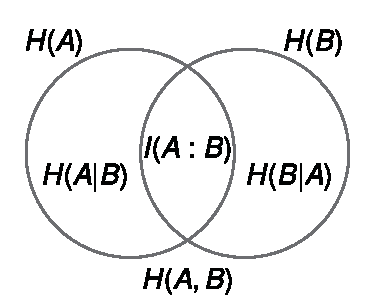
\includegraphics[width=3 in]{figures/ch3/ven_diag_classical.pdf} } 
%\end{figure}

The translation of the information concepts of Shannon entropy to quantum mechanical states is provide through the definition of the von Neumann entropy. Instead of finding the classical microstates populated by a probability distribution, the von Neumann entropy acts on the density matrix of a state:

\begin{equation}
\label{eqn:svn}
S(\rho) = \mathrm{Tr} \left [ \rho \log[\rho] \right ]
\end{equation}

\begin{figure}
\floatbox[{\capbeside\thisfloatsetup{capbesideposition={right,top},capbesidewidth=3 in}}]{figure}[\FBwidth]
{\caption{\textbf{von Neumann entropy and mutual information.} This Venn diagram graphically describes the total information needed to separately describe the constituents $\{ S(\rho_A), S(\rho_B) \}$, as well as the information they share $\mathcal{I}[\rho_{A:B}]$, and the amount of information that is independent of knowing everything about the other constituents $\{ S(\rho_{A|B}),S(\rho_{B|A})  \}$. Since these are quantum states and not classical ones, the bounds are different than those derived for the Shannon entropy can be difference since $S(\rho_{AB})$ can be zero.\cite{Cerf1996,Horodecki1996,Horodecki2007} The classical  and quantum bounds described in this chapter can be understood from this diagram by taking this global entropy bound into account.} \label{fig:Sven}}
{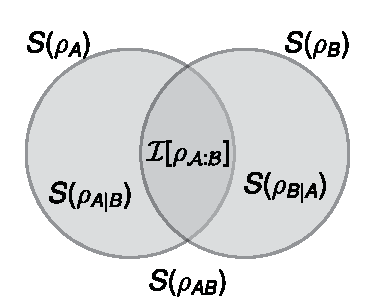
\includegraphics[width=3 in]{figures/ch3/ven_diag_quantum.pdf} } 
\end{figure}

While this definition is basis independent and can be computed as long as one is careful with acting on a matrix with the $\log[]$ function, it is easiest to compute the von Neumann entropy in the diagonalized (or Schmidt basis) of $\rho$ in which the matrix is diagonal.\footnote{This is diagonalization of the density matrix is equivalent to determining the number of pure, many-body quantum states (akin to global microstates) the density matrix populates.} This description of a system by a matrix $\rho$ with the possibility for coherent superposition of many-bodied states fundamentally changes the entropy bounds shown for the classical case. To start with, let us consider the total entropy in a pure state as defined by the Bell state $|\Psi^-\rangle$ above. Since we can choose to rotate $\rho$ to any basis, it is most convenient to express it in the Bell state basis, in which case it is simply a single entry defined by $\rho=|\Psi^-\rangle \langle \Psi^-|$. The fact there is only a single microstate populated means that the total entropy of this system is zero. To understand the significance of this result though, we need to first address the concept of the partial trace of a system -- this is akin to finding the marginal distribution $P_B$ by summing over all possibilities for A : $P_B = \sum_A P_{A,B}$. In the density matrix case this is performed by an inner product with the basis states of system A:

\begin{equation}
\label{eqn:partTr}
\rho_B = \mathrm{Tr}_A [ \rho] = \sum_{a \in A} \langle \phi_a | \rho | \phi_a \rangle
\end{equation}

where $|\phi_a\rangle$ defines a complete, orthonormal basis of subsystem B. If we apply this partial tracing to the originally investigated Bell state $|\Psi^-\rangle$, where $| \phi_a \rangle \in \{ |\uparrow_A\rangle, |\downarrow_A\rangle \}$ then we have constructed $\rho_B$ which is known as the reduced density matrix since it only spans the subspace of spin B:

\[
\rho_B = \frac{1}{2} \begin{bmatrix}
| \uparrow_B \rangle \langle \uparrow_B | & 0  \\
0 & | \downarrow_B \rangle \langle \downarrow_B | \\
\end{bmatrix}
\]

The partial trace, conceptually, is considered the ``ignoring" of information present in the other subsystem, in this case the orientation of spin A. The originally pure, entropically zero many-body state $\rho$ is now locally a completely mixed state with $S(\rho_{B})=\log[2]$. This result elucidates the difference in entropy bounds of the quantum case as compared to the classical one: $S(\rho)$ is no longer bounded from below by $\argmax\{S(\rho_A), S(\rho_B) \}$ and the maximum mutual Information has a much larger upper bound $0\leq I(A:B) \leq S(\rho_A)+S(\rho_B)$.

This regime of $S(\rho) <  S(\rho_A), S(\rho_B)$ is often used to identify the qualitative statement of \emph{entanglement} for a state and defines that some of these correlations are quantum in origin. There are several significant remarks to be noted about such systems. This enhancement of the maximally available mutual information between two subsystems is why entanglement is considered an important and exploitable resource for quantum information and quantum computation purposes\cite{nielsen2010}. Another important observation is that in the case of a pure quantum state, the entropy observed for a subsystem is entirely generated by the loss of information related to the initial coherent, many-body superposition of the state. Lastly, these states are not trivial to generate. This is for two reasons: 1) the many-body state has to start off as a relatively pure one\footnote{In comparison with the locally generated entropy from the partial trace.} and then 2) become correlated such that it is inseparable and therefore entangled. As it will turn out, unitary evolution of an initially separable, pure quantum state through a phase transition is one way generate such entangled states\S \ref{sec:sfmi}, \ref{sec:ising}, \ref{sec:ch4}.

\subsection{Entanglement and quantum phase transitions}

From the previous brief discussion of phase transitions: the growth of correlations near the critical point seems like a clear and natural manifestation of entanglement if the phase transition is a quantum one. However the exact relationship can be a bit subtle. In the case of a $T=0$ phase transition, the system is described by a single eigenstate, namely the ground state, and therefore has zero total entropy. The generation of correlations in the ground-state near the phase transition will make it inherently inseparable and therefore generate entropy among its subsystems -- which indeed makes them entangled on a qualitative level\cite{Vidal2003,Amico2008,Sachdev2011}. 

However, some of the same notions, such as diverging correlation lengths at the critical point, do not straight-forwardly manifest in a quantitative way for the discussed entanglement metrics. For instance, the entropy of a single spin in a many-spin state does not necessarily relate to the number of other spins with which it is correlated. The local entropy is bounded from above by $\log[2]$ and therefore the entanglement of the individual spin with the rest of the system can be distributed arbitrarily via its correlations as long as it respects this bound. This is often referred to as the ``monogamy" of entanglement and refers to the fact that there is a finite amount of this resource that can be distributed among the system. If two spins are maximally entangled, as in the case of the Bell state $|\Psi^-\rangle$, then for them to become entangled with a third spin, they must inherently reduce some of the entanglement they initially shared with one another, even though they may still be just as ``correlated". This property is particularly important when attempting to evaluate the length scale over which entanglement is distributed in a quantum system at a quantum critical point. The first numerical studies addressing this problem, while finding a familiar universal scaling behavior of correlations at the critical point, had difficulty defining the properties of the length scale over which entanglement was spread in the system \cite{Osterloh2002,Osborne2002,Amico2008}.\footnote{This was partially compounded in difficulty due to the wide number of numerical metrics meant to quantify entanglement and the fact that the monogamy of entanglement made many entanglement measures peak around but not necessarily at the transition.} Further studies showed that by always partitioning the system into two macroscopically large subsystems (known as a bipartition), rather than looking at the entanglement between two individual spin subsystems, provided a direct relation of the correlation length to the entanglement entropy near the critical point\cite{Vidal2003}. The entropy for the ground-state transitions was found to scale with the area \cite{Eisert2010}, or boundary, of the subsystem due to the finite correlation length $\xi$ in the system(see Fig.~\ref{fig:areaLaw}).


\begin{figure}
\floatbox[{\capbeside\thisfloatsetup{capbesideposition={left,top},capbesidewidth=3 in}}]{figure}[\FBwidth]
{\caption{\textbf{Area law in ground-state phases.} As demonstrated in \emph{Vidal, et al.}, the entanglement entropy due to a bipartition of the total many-body system into subsystems $\rho_A,\rho_B$ realized a scaling relationship known as an area law. This area law determined that the amount of entanglement entropy probed by the bipartition scaled linearly with the boundary size $\propto l^{D-1}$ of the bipartition rather than the volume $\propto l^D$ for dimension D. This area law's relation to the correlation length was found in critical systems by a logarithmically slow divergence of the entropy with system size $l$ inherited from the diverging correlation length $\xi$.} \label{fig:areaLaw}}
{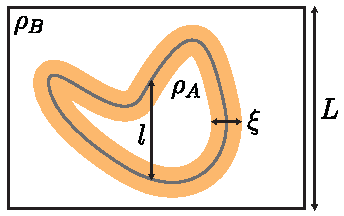
\includegraphics[width=3 in]{figures/ch3/philipp_area_law_cartoon.pdf} } 
\end{figure}

Despite the ubiquitous use and study of entanglement in theoretical physics, current traditional condensed matter experiments do not have a direct probe for measuring it. In a few other similar AMO experiments, entanglement has been probed via entanglement witnesses\cite{Bouwmeester1999}: specifically constructed observables that probe inseparability of a quantum state that violates a particular bound.  Such witnesses are state-specific and do not necessarily scale in a meaningful way with the degree of entanglement in the state. In systems of trapped ions\cite{Haffner2005} and superconducting qubits\cite{Neill2016}, an exhaustive reconstruction of the entire density matrix can be performed, known as state tomography, from which the entanglement entropy can be directly computed. There is not a know scheme for mapping this technique to lattice systems of itinerant particles. Instead, we will demonstrate the use of a many-body interference technique that forgoes the aforementioned techniques. We use this technique to investigate the entanglement developed in ground-state phase transitions\cite{Ekert2002,Moura2004,Palmer2005,Daley2012}. Recently, a new method involving measuring the variation in observable outcomes after random quenches on a single realization have also been demonstrated to measure entanglement entropy\cite{Brydges2019}.

\section{Superfluid-to-Mott-insulator transition}
\label{sec:sfmi}

The superfluid to Mott-insulator transition is one of the most celebrated manifestations of a quantum simulator generating and measuring a quantum phase transition \cite{Greiner2002,Bakr2010,Sachdev2011}. While these experiments were able to explore the properties of the different quantum phases and probe the local order parameter, they were unable to directly measure the entanglement generated in the system. In this experiment, we directly measure the global and local purities of a finite size system in the Bose-Hubbard model through a many-body interference technique \cite{Ekert2002,Moura2004,Palmer2005,Daley2012,Kaufman2014,Islam2015,Kaufman2016}. This purity measurement allows us to directly compute the second-order R\'enyi entropy:

\begin{equation}
\label{eqn:s2}
S_2 (\rho) = -\log [ \mathrm{Tr} [\rho^2] ]
\end{equation}

 which is a quantitative lower bound to the more traditional von Neumann entropy. The same inequalities used for the discussion of the von Neumann entropy above additionally apply to the R\'enyi entropy for measuring entanglement in a system: 
 
 \begin{eqnarray}
 S_2 (\rho) < & S_2 (\rho_A) \\
 S_2(\rho)  < & S_2 (\rho_B)
 \end{eqnarray}

The technique used to measure the R\'enyi entropy relies on the interference of two identical but independent quantum many-body states. This allows one to extract observables that are quadratic in the density matrix which is used here to access the system purity\cite{Ekert2002,Moura2004,Bruni2004,Palmer2005,Bovino2005,Walborn2006,Schmid2008,Daley2012}. The capability to directly measure the R\'enyi entropy is a powerful technique for several reasons: i) it does not rely on violating particular correlation measurement inequalities such as the Clauser-Horne-Shimony-Holt (CSCH) inequality\cite{Horodecki1996,Bovino2005}, ii) quantum state tomography requires a measurement of a prohibitively large Hilbert space and has no known scheme for itinerant systems, iii) in principle requires few measurements to verify low entropies and can be quickly used to bound the global purity of a state. The exact experimental implementation of this technique is thoroughly detailed in \emph{Islam et al.}\cite{Islam2015, Preiss2015, Lukin2018Th} and is not extensively discussed here. The results presented below not only directly measure the development of entanglement in a quantum system, but provide some instructive insights on its origin.

The experiment begins in a Mott-insulating state with unity filling ($U \gg J$) in a finite 1D system of 4 sites. This means that the initial many-body state is described by a product state of exactly one atom per-site:

\[
|\Psi_{MI} \rangle = \prod_{i=1}^{L=4} \otimes | 1_i \rangle
\]

Since this state is a product state, it is inherently separable and therefore unentangled \footnote{There is a common use of the phrase ``strongly-correlated" when referring to the Mott-insulating state which would appear unjustified given the above description. However, as a point of clarification, remember that the concept of entropy from entanglement is always with respect to a given partitioning of the system, while, for any given partition, the metric is basis invariant. In the case of a Mott-insulator, any real-space separation of many-body state generates no entropy.} and both the sub-systems and full-system are pure. As the ratio of $U/J$ is reduced towards the superfluid regime ($J\gg U$) the ground-state becomes a spatially delocalized state:

\[
|\Psi_{SF} \rangle \propto \left ( \sum_{i=1}^{L=4} a^\dagger_i \right )^{\otimes N=L} |vac\rangle
\]

The superfluid ground state with a finite particle number is spatially delocalized and therefore is inseparable among the lattice sites which leads to entanglement entropy when measuring the purity of a subsystem. The R\'enyi entropy measurements shown in Fig.~\ref{fig:sf_mi_fig} show that on the superfluid side of the transition there exists verifiable entanglement among all possible subsystem sizes and partitions. 

\begin{figure}[t!]
		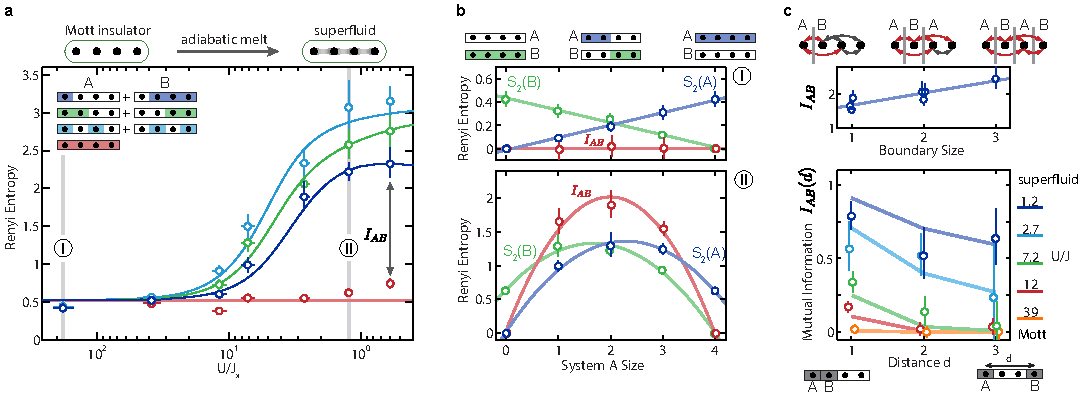
\includegraphics[width=\columnwidth]{figures/ch3/sf_mi_data/fig5.pdf} 
		\caption{\textbf{Measured R\'enyi entropy in the Mott-insulating-to-superfluid transition. a)}  The measured global and subsystem entropies are shown for various partition volumes and arrangements. The area between the subsystem entropies and the global entropies quantify the amount of mutual information generated in the system during the adiabatic ramp to the superfluid state. Note that the entropy inequality that would determine the bound on entanglement in this plot lies close to $1$. The different partitions shown are to illustrate the difference area versus volume laws. \textbf{b)} Illustrates the extensive, volume law scaling, of the background classical entropy injected in the system through residual heating or non-unity fidelity interference contrast. \textbf{c)} The top plot demonstrates the area law behavior of the entropy with partitioning of the subsystems. The lower plot demonstrates the decrease in correlations as a function of distance between non-bipartite subsystems -- as would be expected from a decaying correlation length.  All solid lines in \textbf{a,c} are numerics performed by exact diagonalization. The error bars are the s.e.m. }
		\label{fig:sf_mi_fig}	
\end{figure}

The many-body interference technique performed here shows the measurable development of entanglement entropy. It additionally illustrates its versatility as a technique by its capability to measure variable subsystems sizes and arbitrary partitioning in real-space as a single measurement scheme. Note that while these measurements indeed perform a remarkable job in measuring entanglement, it does not seem to follow the intuition we developed and discussed in the previous section for quantum phase transitions. The reason for this stems from the fact that the system has a conserved particle number that manifests as strong, inherent particle number correlations between a subsystem and the remainder. As an example, imagine a subsystem of one-site. This single-site can have only $N+1$ possible microstates bounded by the total particle number: $0\leq \hat{n}_i \leq N$. However, more importantly, due to the particle number conservation, there are no coherences in the single-site reduced density matrix and it is purely a diagonal matrix. This is because the sub-systems are a bipartition of the total system and therefore the number of atoms in the two subsystems are unique numbers $n_A$, $n_B = N-n_A$. This is actually not a generic feature of the superfluid state, and is dependent upon having a conserved particle number. In the limit of the superfluid being composed of a product of local coherent states:

\[
|\Psi_{SF}\rangle = \prod_i |\alpha_i \rangle 
\]

the total particle number is not conserved, the state is an eigenstate of the Bose-Hubbard model, and a product state of the lattice sites. However, for this experiment where we start in a Mott-insulating state, one must always start with a number of atoms that is commensurate with the lattice size.  Therefore, it is not possible to have a coherent superposition of total particle numbers which is required by this coherent state superfluid.

Schemes have been developed for this protocol that probe only the entropy related to the diverging correlation length at the transition that effectively remove the correlations from fixed global particle number \cite{Wiseman2003,Melko2016}. This entanglement that follows our intuition of quantum phase transitions, however, is rather small. In the absence of this modal entanglement from particle delocalization, this particular transition would make experimental demonstration of entanglement entropy very challenging. 

\section{Ising model phase transition}
\label{sec:ising}

This section starts with a brief overview of another canonical phase transition that occurs in the  Ising model with both longitudinal and transverse magnetic fields. Importantly, the implementation of this model in our Bose-Hubbard system has characteristics that are more akin to the phase transition behavior expected without any conservation rules such as conserved particle number. Through the use of our DMD, we can access the full-counting statistics of the quantum state in the Fock basis. This allows us to directly probe the order parameter of the quantum phase, the single-site entropy, and the reversibility of the transition which probes its overall adiabaticity and purity.

This model has been previously realized in this same experimental apparatus\cite{Simon2011} and is more thoroughly discussed in the following theses\cite{Bakr2011,Ma2014}.  The mapping from the Bose-Hubbard model to a spin model was first proposed by \emph{Sachdev et al.}\cite{Sachdev2002} and is accomplished by working in a reduced Hilbert space via a strong potential gradient in the optical lattice. The primary ingredients of this mapping are shown in Fig.~\ref{fig:IsingMap}.

\begin{figure}[t!]
		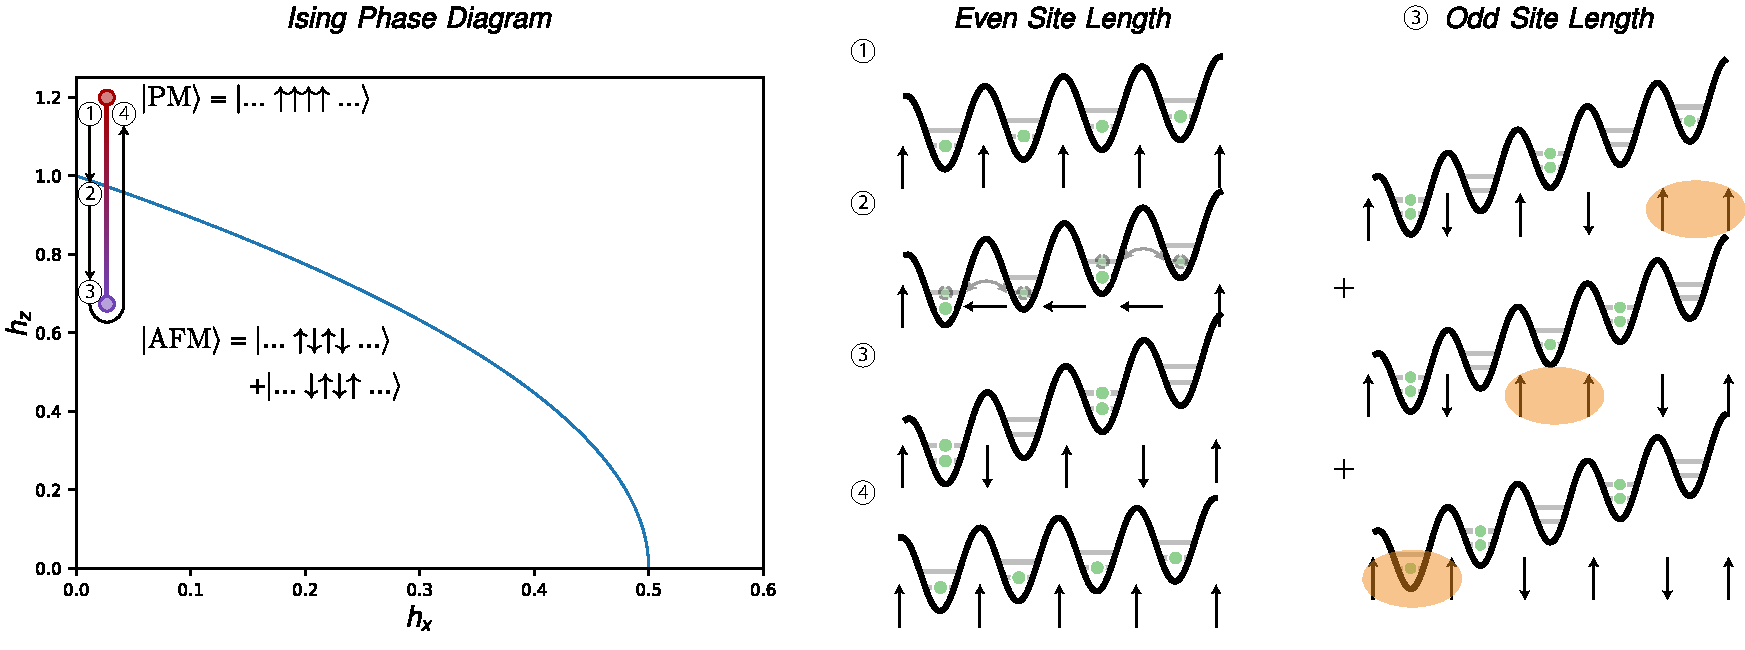
\includegraphics[width=\columnwidth]{figures/ch3/ising_data/AFM_ising_map.pdf} 
		\caption{\textbf{Bose-Hubbard to Ising model mapping. a)}  The phase diagram is shown on the left with the adiabatic path taken that leads to the transition from the paramagnetic phase $|PM\rangle$ to the antiferromagnetic $|AFM\rangle$ ones. The mapping of on-site occupations to spin alignment is shown for total system sizes of both even- and odd-site lengths. \textbf{b)} These boundary conditions only effect the $|AFM\rangle$ states. In the even-site regime there is a single ground-state orientation, while in the odd-site regime the ground state contains a delocalized domain wall (denoted as the orange bubble).}
		\label{fig:IsingMap}	
\end{figure}


This mapping starts in a regime where $U\gg J$,  $U/2<E<U$\footnote{The lower bound forgoes the contribution of second-order hopping processes that incorporate states outside of the prescribed basis for a faithful mapping to the Ising model. This was found to be a necessary step since these second-order processes provided a non-negligible fraction of population into these states.}: $U\approx 410 \mathrm{Hz}$ and $J=6\mathrm{Hz}$. This realizes a set of eigenstates that are approximately described by the Fock basis. The gradient potential, $E$, starts at a low value $E_{-} \approx 307\mathrm{Hz}$ is then increased till $E_+\approx 512 \mathrm{Hz}$. This ramp passes through a regime where every site is on-resonance with its neighbor when the offset is equal to the energy $U$. However, the important aspect of these dynamics arise from the collusion of all the particles in the system such that they transfer in a many-body coherent way and the system remains in the global ground state.  All Bose-Hubbard-to-Ising-model mappings are listed in Appendix: \ref{appendix:Ch3Cal}. After following the mapping prescribed by \emph{Sachdev et al.}\cite{Sachdev2002}, the resultant spin Hamiltonian is given by: 

\begin{equation}
\label{eqn:isingHam}
H=J \sum_i S^i_z S^{i+1}_z - (h_z + \delta^i_z)S^i_z - h_x S^i_x
\end{equation}

where the transition in this Hamiltonian is approximately at $h_z = 1 - 0.66 h_x$.

Importantly, the ground states of the system are approximately locally factorable on either side of the transition. In the paramagnetic (PM) phase, which is the unity filling Mott insulator we start with, the system is separable both in the spin mapped Hilbert space and the bare Hilbert space of lattice-site occupations. The spin mapping here is that $|n_i=1 \rangle \rightarrow | \uparrow \rangle $.  After going through the $E\approx U$ resonance, atoms that hop to their neighboring site will be considered the spin-flipped atoms. This implies that lattice-site occupations $|n_i= 0 \rangle \rightarrow | \downarrow \rangle $, while $| n_i = 1,2 \rangle \rightarrow | \uparrow \rangle$. This phase is known as the antiferromagnetic (AFM) phase of the transition. This corresponds to a charge-density wave in the bare basis of on-site occupation number.

While the initial state is independent of boundary conditions, the final state is sensitive to the bounds of the system. In the case of periodic boundary conditions, the final state is a superposition of two possible AFM configurations: $|\Psi_{AFM}\rangle = | ... \uparrow \downarrow \uparrow \downarrow ... \rangle + | ... \downarrow \uparrow \downarrow \uparrow ... \rangle $. While this case is useful theoretically for computation, it is rather unphysical. The experiment is always a finite size system with open boundary conditions. This imposes two generic types of ground states that depend upon whether the system size includes an even or odd number of lattice sites (Fig.~\ref{fig:IsingMap}). In the case of an even number of lattice sites, there is a single state for both the paramagnetic and antiferromagnetic ground states. This is the case shown in Fig.~\ref{fig:ising_N4N5}\textbf{a} for an $N=4$ site system. In contrast to previous work\cite{Simon2011}, we now resolve the on-site number which enables us to directly measure the exact ground state for the PM or AFM phases on either side of the transition and the order parameters (e.g. N\'eel order parameter): 

\begin{equation}
\label{eqn:Neel}
\left \langle \hat{\mathcal{O}}_{AFM} \right \rangle = \left \langle \left (  \sum_j (-1)^j \hat{s}_j^z \right )^2  \right \rangle
\end{equation}

Additionally, since we are working with a conserved particle number for a finite size system, the correlations related to the particle number distribution on a single-site can be directly related to the single-site entropy. This provides a metric with which to probe the enhanced quantum fluctuations that occur at the critical point of the phase transition which are also shown in Fig.~\ref{fig:ising_N4N5}.

\begin{figure}[t!]
		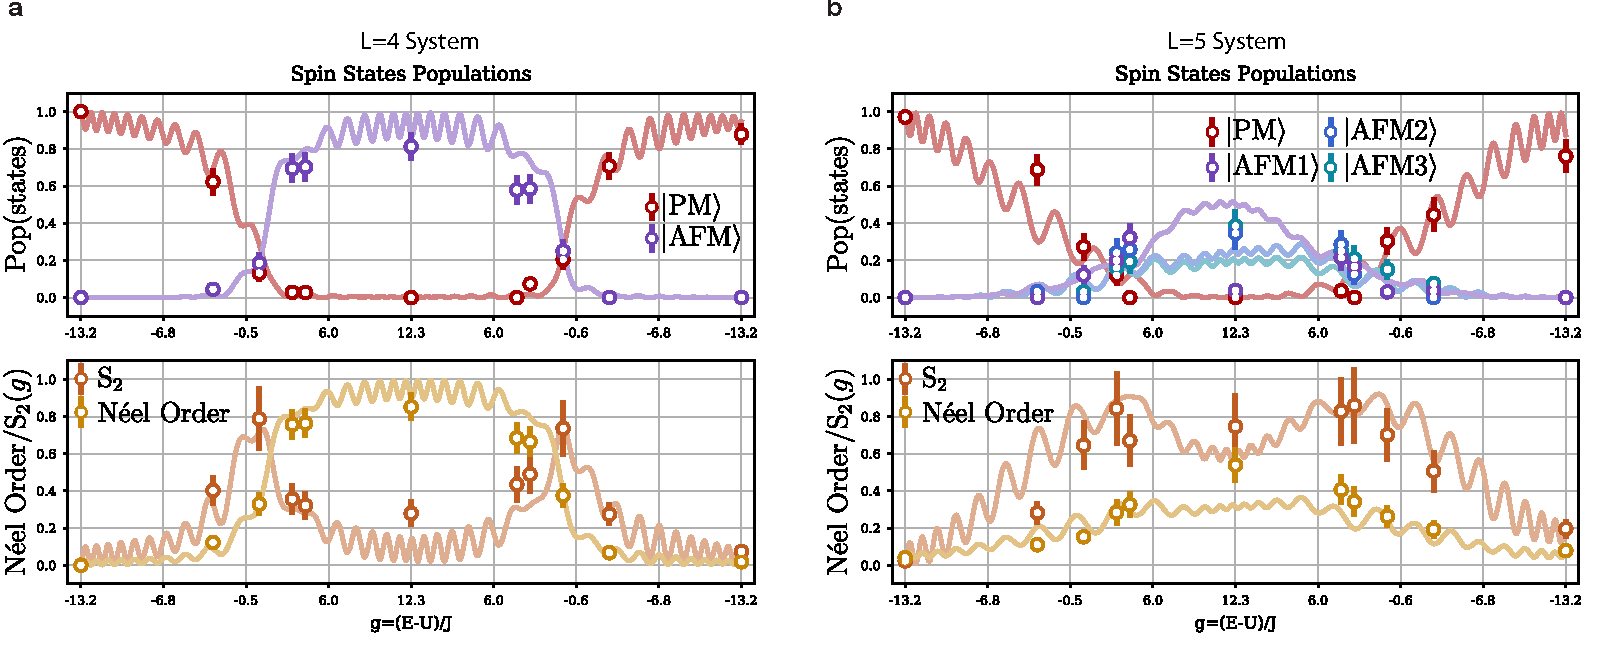
\includegraphics[width=\columnwidth]{figures/ch3/ising_data/IsingN4N5Combo_2v2edit.pdf} 
		\caption{\textbf{Measured population in magnetic states, order parameter, and single-site entropies. a)}  The top plot shows the population in the paramagnetic state and antiferromagnetic state as a function of the tuning parameter $g$ for the $N=4$ system. The system is shown ramping through the transition and back to demonstrate the adiabaticity of the process and bound the amount of entropy generated at the transition due to diverging correlation length at the critical point. The lower plot shows the increase of entropy near the critical point (orange) and the measured N\'eel order (blue) that occurs in the AFM phase. \textbf{b)} The top plot shows the population in the paramagnetic state and antiferromagnetic states as a function of the tuning parameter $g$ for the $N=5$ system. Note that now the three possible AFM states that admit a single domain wall are now plotted. This inherint domain wall incurs a reduction in the order parameter presented in the lower plot and the increase in the entanglement entropy in the AFM phase. All solid lines are exact numerics performed by Trotterized time evolution. The error bars are the s.e.m.}
		\label{fig:ising_N4N5}	
\end{figure}

In the case of an odd number of lattice sites, there is always a single domain wall somewhere in the system due to the frustration of trying to anti-align all neighboring spins. This leads to an AFM ground state composed of the $N-2$ possible configurations with a single domain wall. This superposition of this domain wall leads to an additional residual entropy in the AFM phase that can be seen by both a non-zero entropy in the single-site entropy and a reduced N\'eel order parameter. This is shown for an $N=5$ site system in Fig.~\ref{fig:ising_N4N5}\textbf{b}.

%
%\begin{equation}
%\label{eqn:domainWall}
%\langle \hat{\mathcal{O}}_{DW} \rangle = \left  \langle \sum_j  \left (1+\hat{s}_j^z \hat{s}_{j+1}^z \right )  \right \rangle
%\end{equation}


We scale the system size for both the even and odd site cases to see how the transition depends upon the total system size. The finite size of the system is related to the minimum gap in the system and is associated with a shrinking of the critical region(Fig.~\ref{fig:qpt}) that lies between the two quantum phases\cite{Sachdev2011}. This shrinking gap size with system size will require longer ramp times to maintain adiabaticity during transition. The on-site atom number resolution affords us the ability to measure the local order parameter and peak single-site entropy of this transition for system sizes $4\leq L \leq 8$ which are plotted in Fig.~\ref{fig:n_scale}.


\begin{figure}[t!]
		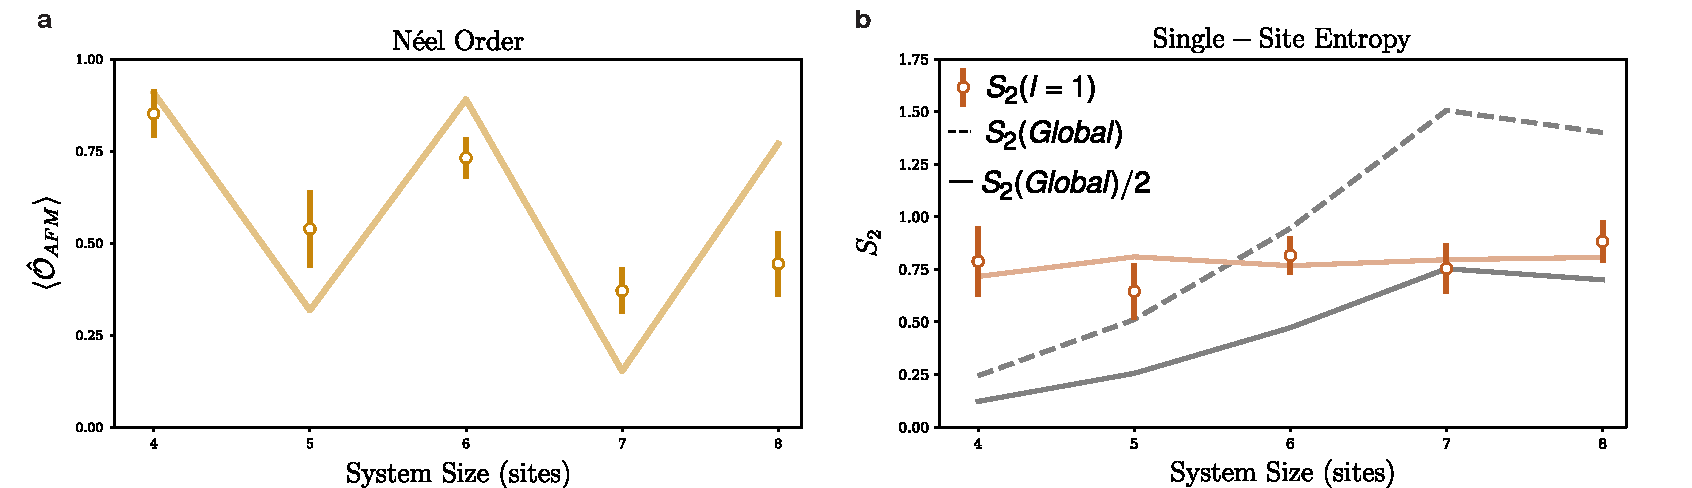
\includegraphics[width=\columnwidth]{figures/ch3/ising_data/SingleParamEdit_2v2edit.pdf} 
		\caption{\textbf{System size scaling: order parameter and single-site entropy. a)} The N\'eel order parameter is plotted for the tuning parameter ($g\gg g_c$) deep in the AFM phase as a function of system size. The staggered structure reflects the domain wall excitations in the odd-site system size ground states. The additional suppression of the expected order parameter value for the even-site system reflects the shrinking gap at the critical point that restricts the maximum correlation length possible in a finite time ramp. \textbf{b)}  The single-site entropy remains nearly maximized for all explored system sizes. Importantly, we can use this to distinguish whether the system's change in order arise due to quantum fluctuations by comparing this entropy the global purity estimates (black solid and dashed lines). All solid,colored lines are exact numerics performed by Trotterized time evolution. The error bars are the s.e.m.}
		\label{fig:n_scale}	
\end{figure}

To determine whether the entropy measured at the critical point is due to entanglement, we have to compare this single-site entropy to the global entropy of the system. In the even site case, the ground state on either side of the phase transition is approximately an eigenstate of the many-body Fock state in our system and enables us to directly estimate an upper bound on the global entropy in the system by simply estimating the purity from the  diagonal of the measured density matrix (\ref{eqn:classicalPurity}) in an arbitrary basis. 

\begin{equation}
\label{eqn:classicalPurity}
\mathrm{Tr} [\rho^2] \leq \sum_i \rho_{i,i}^2
\end{equation}

In the case of an odd-site system, it is more insightful to reverse the transition back to the initial state. By estimating the entropy from either one of these cases at the end of the initial sweep, we can make a stricter statement about whether the entropy at the critical point is due to the entanglement of the quantum state. We see that based upon the estimate on the global purity after reversing the dynamics that we can strictly make this statement about this transition up to the system size $N\leq5$. Although, if we assume that the non-adiabaticity of the ramp that leads to this lack of purity occurs from ramping through the transition twice, then a closer estimate would show this to be true for system sizes $N\leq7$.

There is an additional influence on these dynamics that derives from residual disorder in the optical lattice. Inhomogeneous potential offsets on individual lattice sites correspond to local variation in fields $h_z$ in (\ref{eqn:isingHam}). If these local fields are on the order of the coupling strength between sites, the minimum gap will significantly decrease and one can effectively think of several, nearly, disconnected chains undergoing the transition. These will create a set of chains that are effectively incoherently populated with respect to one another and may not reversibly map back to the PM state.

A last comment to be made from looking at the odd-numbered lattice sites in Fig.~\ref{fig:ising_N4N5} is that not all single-domain wall states are equivalent in the AFM phase. This actually becomes an intuitive outcome of this frustration if one considers the single-domain wall like a single-particle or excitation in a box. The wave function of this single-excitation on top of the AFM background will have a ground state minimized by its kinetic energy within a confined volume -- akin to the typical cosine solution for a single-particle in a box.

\section{Discussion}

The demonstrated measurements of entanglement entropy in ground-state phases provide a basis for experimental exploration of entanglement and quantum criticality in ground-state quantum phases. The microscopic access available to the system allows for a direct measurement of the microscopic entropy, the order parameter, and could be extended to extract the corresponding correlation length in the system. Additionally, other proposals for multipartite entanglement witnesses through the quantum Fisher information can be applied that also have access to the global entropy through dynamic susceptibilities \cite{Hauke2016}. These techniques could be applied to measure the Kibble-Zurek mechanism that governs the expected critical behavior \cite{Polkovnikov2005,Zurek2005}. Experimentally, such scaling behavior has been seen for both strongly interacting system and those captured by a mean-field approach\cite{Endres2012,Anquez2016,Clark2016,Keesling2019}. 

Lastly, this chapter has only focused on the concept the role of entanglement and fluctuations in the context of equilibrium systems. In all of the successive chapters of this thesis, the same concepts will be used and applied for pure quantum systems that that are far from equilibrium. This will inherently involve eigenstates other than the ground-state of the system. We will now focus on the characteristic behavior of these excited eigenstates and how they, too, harbor many-body physics similar to the concepts discussed here.
